%% LyX 1.5.5 created this file.  For more info, see http://www.lyx.org/.
%% Do not edit unless you really know what you are doing.
\documentclass[11pt,a4paper,english,conference,compsoc,twoside,twocolumn]{IEEEtran}
\usepackage[T1]{fontenc}
\usepackage[latin9]{inputenc}
\usepackage{float}
\usepackage{graphicx}

\makeatletter
%%%%%%%%%%%%%%%%%%%%%%%%%%%%%% LyX specific LaTeX commands.
%% Because html converters don't know tabularnewline
\providecommand{\tabularnewline}{\\}
\floatstyle{ruled}
\newfloat{algorithm}{tbp}{loa}
\floatname{algorithm}{Algorithm}

%%%%%%%%%%%%%%%%%%%%%%%%%%%%%% User specified LaTeX commands.
%% LyX 1.5.5 created this file.  For more info, see http://www.lyx.org/.
%% Do not edit unless you really know what you are doing.

\usepackage{geometry}

\geometry{verbose,tmargin=2.5cm,bmargin=2.5cm,lmargin=2.5cm,rmargin=2.5cm}

\setlength{\columnsep}{0.6cm}
\setlength{\columnwidth}{7.7cm}

%%%%%%%%%%%%%%%%%%%%%%%%%%%%%% LyX specific LaTeX commands.
%% Because html converters don't know tabularnewline

\author{
\IEEEauthorblockN{Li Lin}
\IEEEauthorblockA{Crimsonwing Malta\\
28, Moroni street, Gzira, Malta\\
Email: lliz003@um.edu.mt}
\and
\IEEEauthorblockN{Kevin Vella}
\IEEEauthorblockA{Department of Computer Science\\
University of Malta\\
Email: kevin.vella@um.edu.mt}
}

\makeatother

\makeatother

\usepackage{babel}

\begin{document}

\title{Fast User-Level Inter-thread Communication, Synchronisation}

\maketitle
\begin{abstract}
This project concerns the design and implementation of user-level
inter-thread synchronisation and communication algorithms. A number
of these algorithms have been implemented on the SMASH user-level
thread scheduler for symmetric multiprocessors and multicore processors.
All inter-thread communication primitives considered have two implementations:
the lock-based implementation and the lock-free implementation. The
performance of concurrent programs using these user-level primitives
are measured and analyzed against the performance of programs using
kernel-level inter-thread communication primitives. Besides, the differences
between the lock-based implementations and lock-free implementations
are also analyzed. 
\end{abstract}

\begin{IEEEkeywords}
Lock-free, multithreading, synchronisation
\end{IEEEkeywords}

\section{Introduction}

SMASH\cite{4} is a user-level thread system running on Linux. It
was originally developed by Kurt Debattista in 2001. Since then it
has been actively developed in the University of Malta. Before this
project, it lacked user level inter-thread communication primitives
such as mutexes\cite{8}, semaphores\cite{8}, etc. As a result, whenever
these primitives are needed, one has to use the one offered by the
kernel. This may lead to some performance degradation. Because first
since these primitives are implemented in the kernel, the operations
on them usually involve system calls which are expensive. More importantly,
if a user-level thread has to block on a primitive, the underlying
kernel thread is also blocked, hence no other user-level threads can
run on that kernel thread. We try to solve these problems by implementing
inter-thread communication primitives at user level.

The main objective of this project is to implement a inter-thread
communication library for a particular implementation of SMASH, and
to find out how these primitives affect the performance of the SMASH
system. Since these primitives are shared objects among threads, to
guarantee the consistency of these objects, certain synchronization
mechanisms have to be used. When implementing these synchronization
algorithms, there are two approaches: the lock-based approach and
the lock-free approach. In lock-based algorithms, critical sections
are protected by some forms of locks. A typical example is the spin
lock, which is widely used on SMP systems\cite{8}. In this project,
all lock-based designs use spin locks.

Usually, lock-based algorithms are easy to design. However, lock-based
algorithms have problems like dead (or live) lock, priority inversion
and the convoy effect. These problems can be solved with lock-free
algorithms\cite{9}. A concurrent algorithm is lock-free if after
a finite number of execution steps, at least one of the participating
threads progresses to the final goal. Lock-free algorithms are free
of dead locks, but some particular threads may be delayed indefinitely.
A stronger concept is the wait-free algorithms. An algorithm is wait-free
if after a finite number of steps, all participating threads can finish.
In this project, each inter-thread communication construct has a lock-free
implementation.


\section{Design and implementation}

All communication primitives introduced in this project have their
lock-based implementations in which critical sections are protected
by spin locks. These lock-based implementations are very simple, hence
we will not discuss their details. In contrast, their lock-free designs
are complicated. Therefore in this paper, we mainly focus on them.
In addition, we implemented a wait-free CSP communication channel\cite{6}
designed by Vella\cite{3}.


\subsection{Lock-free Mutex}

%
\begin{algorithm}[H]
 

\caption{Lock free Mutex}


\begin{footnotesize} L1~~struct lockfree\_mutex \{

L2~~~~int lock;

L3~~~~int counter;

L4~~~~struct fifo waiting\_queue;

\}\\


L5~~FetchAndAdd(\&mutex->counter,1);

L6~~~~if(Swap(\&mutex->lock,LOCKED))

L7~~~~~~FetchAndAdd(\&mutex->counter,-1);

L8~~~~else \{

L9~~~~~~enqueue(thread\_self,mutex->waiting\_queue);

L10~~~~~schedule the next runnable thread;

L11~~~~\}\\


L12~~counter = mutex->counter;

L13~~~~if(counter == 0)

L14~~~~~~if(!CAS2(<\&mutex->lock,\&mutex->counter>,

~~~~~~~~~~~~~~~~~~~~~~~<0,0>,<1,0>)) \{

L15~~~~~~~~do \{

L16~~~~~~~~~~thread = dequeue(mutex->waiting\_queue);

L17~~~~~~~~\}while(thread == NULL);

L18~~~~~~~~FetchAndAdd(\&mutex->counter, -1);

L19~~~~~~~~enqueue(thread,run\_queue);

L20~~~~~~~\} \end{footnotesize} 
\end{algorithm}


We designed a lock-free mutex in this project. The challenges in the
design are how to modify the status of the mutex and manipulate the
waiting queue concurrently in a lock-free manner. In addition, the
lost-wake-up problem has to be solved. The instruction \emph{Swap}
was used to modify the \emph{lock} field in the mutex. The waiting
queue was adopted from \cite{1}. In order to solve the lost-wake-up
problem\cite{8}, we added to the mutex structure a field \emph{counter}
which represents the number of threads trying to acquire the mutex.
When a thread calls Getmutex function, it first increments the counter
by 1 with the atomic instruction \emph{Fetch\_And\_Add}. Then it tries
to obtain the mutex with \emph{Swap}, if successful, the counter is
decremented by 1 with \emph{Fetch\_And\_Add} again. Otherwise, the
thread blocks on the mutex by inserting itself to the waiting queue.
When a thread calls Releasemutex function, it checks whether the counter
is zero, if so, then the lock field is set to zero, i.e. the mutex
is released. This process is done with \emph{CAS2} to guarantee the
atomicity. \emph{CAS2} fails to release the mutex iff the counter
is non-zero which means there exists threads trying to obtain the
mutex, but they may have or have not inserted themselves into the
waiting queue. Hence, we used an indefinite loop to dequeue a thread
from the waiting queue. The loop terminates if a thread has been successfully
dequeued from the waiting queue. And finally the dequeued thread is
woken up by being inserted into the run queue.


\subsection{Lock-free semaphores}

%
\begin{algorithm}
\caption{The lock-free semaphore}


\begin{footnotesize} L1~~struct sem\_t \{

L2~~~~int counter;

L3~~~~struct fifo waiting\_queue;

L4~~\}\\


L5~~wait(sem\_t s) \{

L6~~~~~ /{*} we may also use FetchAndAdd here, but I suspect
that the following code can improve the latency. {*}/

L7~~~~~do \{

L8~~~~~~~~counter = s->counter;

L9~~~~~\}while(!cas(\&s->counter,counter,counter-1));

L10~~~~~if(counter < 0)

L11~~~~~~~~save the current contex;

L12~~~~~~~~enqueue(thread\_self, s->waiting\_queue);

L13~~~~~~~~switch to the next runnable thread;

L14~~~~~else

L15~~~~~~~~return

L16~~\}\\


L17~~signal(sem\_t s) \{

L18~~~~do\{

L19~~~~~~old = s->counter

L20~~~~~~~~do\{

L21~~~~~~~~~~if( s->counter< 0 )

L22~~~~~~~~~~~~tmp\_thread = dequeue(s->waiting\_queue);

L23~~~~~~~~~~~~if(tmp\_thread == NULL)

L24~~~~~~~~~~~~~~continue;

L25~~~~~~~~~~~~else

L26~~~~~~~~~~~~~FetchAndAdd(\&s->counter, 1);

L27~~~~~~~~~~~~~wakeup(tmp\_thread);

L28~~~~~~~~~~~~~return;

L29~~~~~~~~~else

L30~~~~~~~~~~~break;

L31~~~~~~~\}while(true);

L32~~~~\}while(!CAS(\&s->counter,old,old+1))

L33~~\} \end{footnotesize} 
\end{algorithm}


In the design of our lock-free semaphore, the waiting queue is the
same lock-free FIFO queue as the one used our lock-free mutex. the
counter is modified with \emph{Compare\_and\_Swap} and is allowed
to take negative value. If the counter is negative, then its modules
represents the number of threads that are currently waiting for the
semaphore, but some of them may not have inserted themselves into
the waiting queue. When a thread tries to release a semaphore, it
first reads the counter. If the counter is negative, then it tries
to dequeue a thread from the waiting queue. If it gets a thread successfully,
then it wakes up that thread and increments the counter by 1 with
\emph{Fetch\_And\_Add}, after which the function returns directly
avoiding the outer loop between L18 and L32. However, if it fails
to get a waiting thread, then there are two possibilities: the waiting
thread has not inserted itself into the waiting queue, or the waiting
has been emptied by other threads releasing the semaphore. Therefore,
in the loop between L20 to L31, before the dequeue operation, the
counter is checked first. If it is not negative any more, then the
loop is broken out. In the otter loop, the counter is updated with
\emph{Compare\_and\_Swap}. This guarantees that after the inner loop
is broken out, the counter has not been changed by any other threads,
hence the semaphore can be released safely without the lost-wake-up
problem.


\subsection{Lock-free message queue}

%
\begin{algorithm}
\caption{the lock-free message queue}


\begin{footnotesize} struct message\_queue \{

~~struct lockfree\_fifo {*} queue;

~~cthread {*} waiting\_thread;

~~int waiting\_mark;

\}\\


Fetch\_message(struct message\_queue {*} q) \{

~~while(true) \{

~~~~queue->waiting\_mark = WAITING;

~~~~result = dequeue(q->queue);

~~~~if(result == NULL)

~~~~~~save the current context;

~~~~~~q->waiting\_thread = thread\_self;

~~~~~~switch to the next runnable thread;

~~~~~~continue on wakeup

~~~~else

~~~~~~queue->waiting\_mark = NOWAITING;

~~~~~~reture result;

\}\\


Send\_message(message, struct message\_queue q) \{

~~enqueue(message, q->queue);

~~do \{

~~~thread = swap(\&queue->waiting\_thread,NULL);

~~~if(thread != NULL)

~~~~~queue->waiting\_mark = NOWAITING;

~~~~~wakeup(thread);

~~while(queue->waiting\_mark == WAITING);

\} \end{footnotesize} 
\end{algorithm}


The message queues we implemented are unbounded, multiple sender,
single receiver queues. Unboundedness means that these queues are
potentially capable of storing infinitely many messages. The only
limit is the memory space. Also there can be more than one sender
that sends messages to the queue concurrently, but there is only one
receiver. If the receiver tries to retrieve a message from a empty
queue, it blocks until a sender wakes it up.

In order to implement the lock-free message queue, we use the lock-free
queue from \cite{1} to store messages and add a field \emph{waiting\_mark}
to the queue structure. When a thread tries to fetch a message from
the queue, it first sets the \emph{waiting\_mark} to WAITING to denote
that the receiver is fetching messages. Then it performs the dequeue
operation. If no message is found, then it blocks on the queue. When
a sender sends a message, it inserts the message into the queue, then
check the \emph{waiting\_mark}. If its value is WAITING, then the
sender swaps NULL to the field \emph{waiting\_thread}. If the obtained
value is not NULL which means that the receiver is blocking on the
queue. Therefore the sender inserts the waiting thread into the run
queue. Finally, the field \emph{waiting\_mark} is set to NOWAITING.
Otherwise, the sender repeats the above process until the value of
\emph{waiting\_mark} is NOWAITING.


\subsection{Wait-free channels}

In this project, we also implemented Vella's wait-free CSP channel\cite{3}.
It was designed for KRoC which is an implementation for the OCCAM
2 programming language. The design was totally wait-free, it did not
contain any form of locks or indefinite loops. In the design, the
only special atomic instruction used was \emph{Swap}. For details
of the design, one can refer to \cite{3}.


\section{Results }

The machine we used to conduct the benchmarks is a laptop equipped
with a Intel Core2 Duo 1.83Ghz CPU with 4Mb L2 cache, 2Gb memory.
The operating system is Debian GNU/Linux unstable with Linux kernel
version 2.6.24. The compiler is GCC 4.3. When measuring these benchmarks,
we try to run as few programs as possible, the largest program running
being the X-window system.


\subsection{Mutexes}

We created six identical independent tasks, each of which contains
nothing but a critical section protected by a mutex. In the critical
section, a thread loops to increment a counter which is not shared.
For each critical section, we create ten user-level threads working
on it. The program loops for a number which is defined by GRANULARITY.
We used a pthread mutex and our lock-free mutex to analyze the performance.
It is desirable that the choice of different implementations of user-level
mutexes will not make a significant difference since we are measuring
the performance of the entire system, not that of mutexes.

%
\begin{figure}
\caption{Benchmarks of the system when using different mutexes}


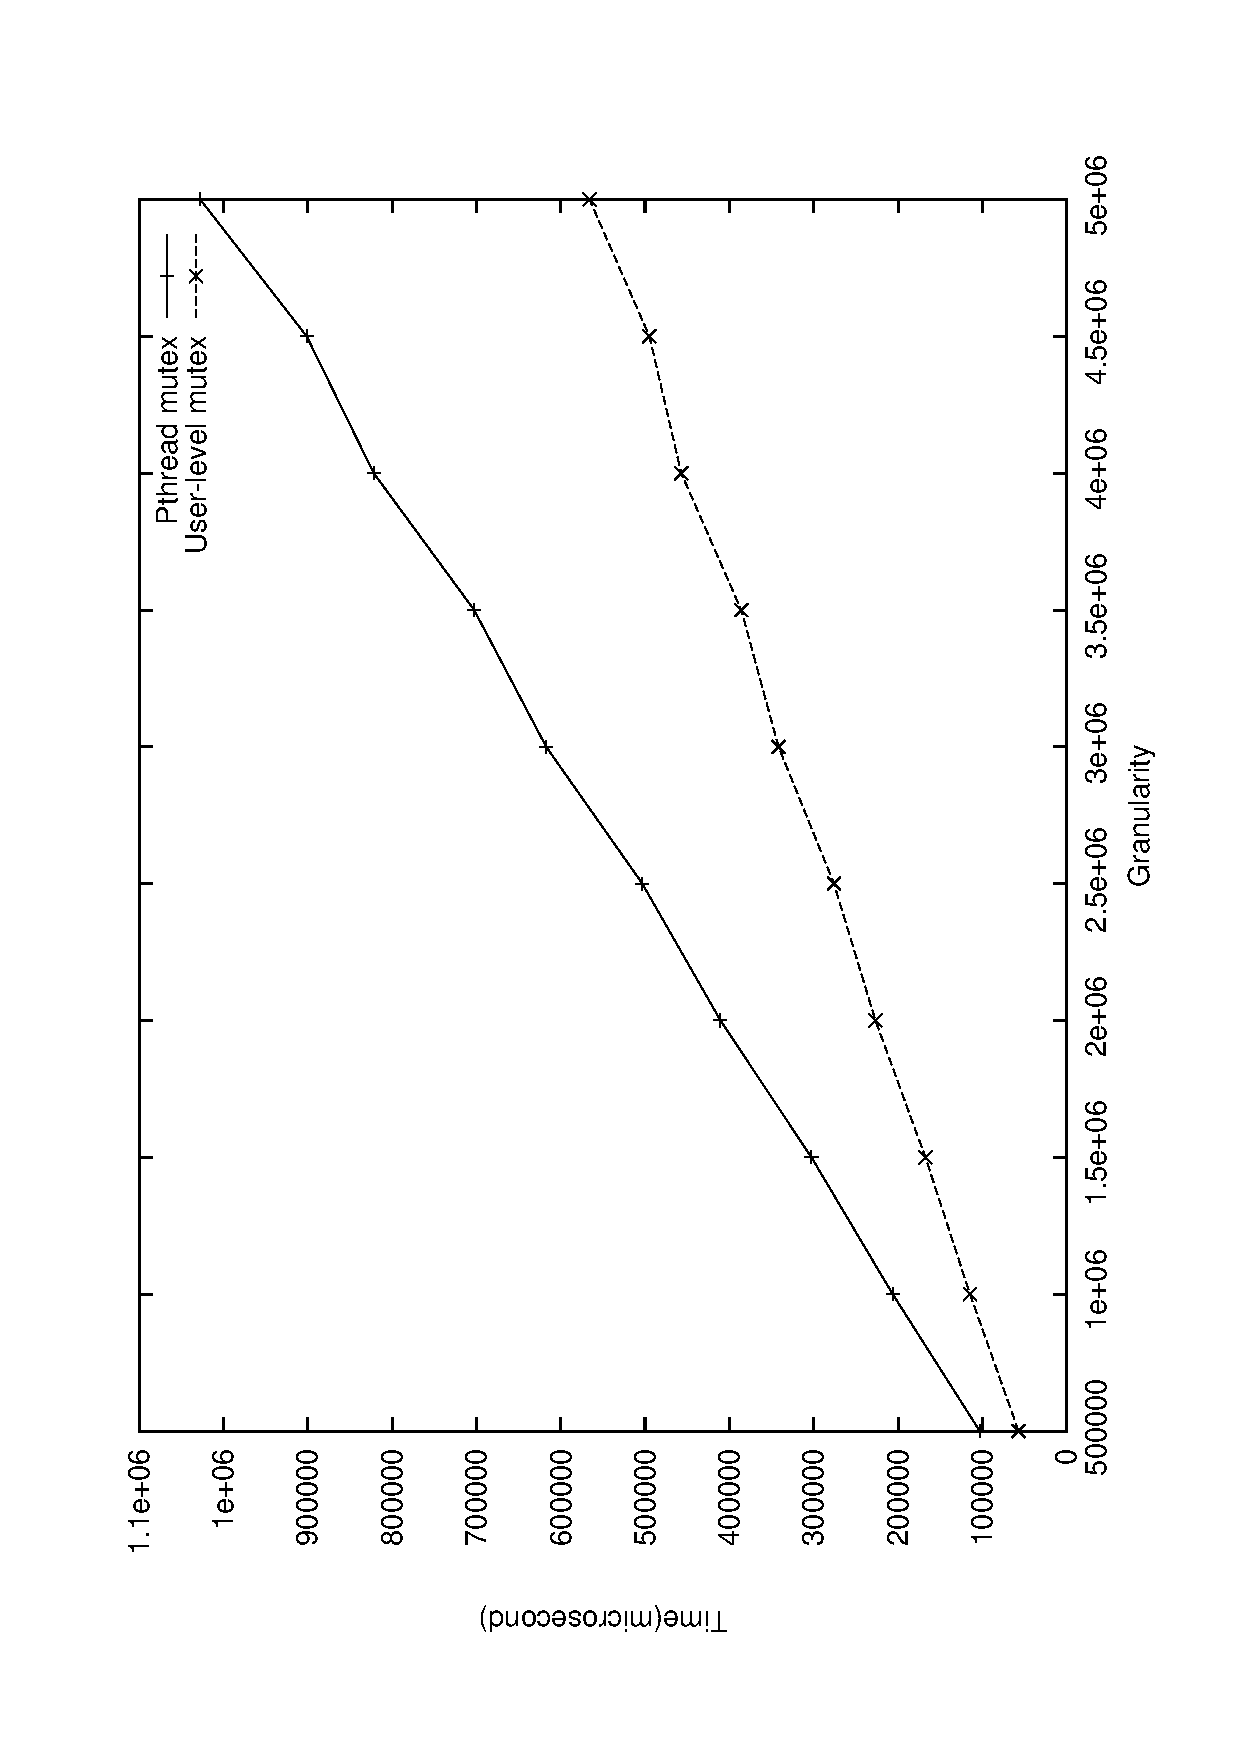
\includegraphics[scale=0.3,angle=-90]{mutex} 
\end{figure}


From the results, we can see that on average, the performance of the
system when using the user-level mutex is twice that when using pthread's
mutex. This is because user-level mutexes never block the kernel threads.
In fact, in the best case, it is possible that when using pthread's
mutex, each kernel picks up a different task to do, therefore, there
is no contention on these mutexes. In this case, we can still get
the same performance as with user-level mutexes. However, in the worst
case these tasks will be processed one by one in a strictly sequential
manner, i.e. we do not benefit from the other CPU at all. This happens
when the two kernel threads always try to work on the same task, so
one of them is always blocked.

Another benchmark is to measure the performance of the function \emph{Getmutex}
and \emph{Releasemutex} when the mutex is not under contention. In
this case, it is not enough to time a single function call to \emph{Getmutex}
since the time of executing the function is not large enough to compensate
the time that is cost by calling the function \emph{gettimeofday()}\cite{5}.
In order to measure the benchmark accurately, we have to perform a
large number of function call to \emph{Getmutex}, then calculate the
average time for a single call. However, this approach is not valid,
because once we call \emph{Getmutex}, it will lock the mutex. Hence,
we call \emph{Getmutex} followed by a call to \emph{Releasemutex},
and we use a loop with 1000000 iterations to execute such a pair,
and then calculate the average time for a single pair.

%
\begin{table}[H]
 

\caption{Benchmark for mutexes(\emph{ns})}


~~~~~~\begin{tabular}{|c|c|c|}
\hline 
Pthread mutex  & Lock-based  & Lock-free\tabularnewline
\hline
\hline 
74  & 95  & 127\tabularnewline
\hline
\end{tabular}
\end{table}


As we can see, the lock-free mutex is slower than the lock-based mutex
for the case in which there is no contention, this is reasonable because
the lock-free mutex uses a lot of expensive atomic operations like
\emph{Fetch\_And\_Add}, \emph{Compare\_And\_Swap} and \emph{Double\_Compare\_And\_Swap}.
In addition, the algorithm is also more complicated, while in contrast,
the lock-based mutex just uses \emph{Swap} and is therefore simpler.
The pthread mutex is the fastest for the uncontended case, because
Linux 2.6 series kernels features a new technique called futex\cite{2,7}
(fast user space mutex). Prior to Linux 2.6, a call to \emph{pthread\_mutex\_lock}
had to enter the kernel and operate on the pthread mutex, then return
to user mode even the mutex is not under contention. But by using
futexes, all operation will remain in user mode for uncontended case
and the pthread mutex on SMP system is also implemented though spin
locks. The code is written directly assembly language and it is manually
optimized, that is why it is the fastest.


\subsection{Semaphores}

%
\begin{table}[H]
 

\caption{Benchmarks of semaphores(\emph{ns})}


~~~~~~~\begin{tabular}{|c|c|c|}
\hline 
Lock-free  & Lock-based  & System\tabularnewline
\hline
\hline 
90  & 96  & 383\tabularnewline
\hline
\end{tabular}
\end{table}


We use the same algorithm as the one used in the above section to
measure the impact of user-level semaphores to the performance of
the SMASH system, the only thing changed is that in this case we use
semaphores initialized to some number to protect the critical section.

Due to the hardware limit, we are not able to measure the benchmark
for a semaphore whose counter was initialized larger than one, because
we only have a dual core machine, hence SMASH will only create two
kernel threads and all user-level threads are run by these two kernel
threads. So if a semaphore is initialized to a number larger than
1, there will not be any contention on the semaphore. As a result,
we only conducted the benchmark with semaphores initialized with 1,
but in this case, the semaphores behave just as mutexes, hence we
have similar result patterns as above.

In fact, on the SMASH system, no matter how many user-level threads
access a semaphore, if the semaphore is initialized to a number smaller
than the number of CPUs (i.e. the number of kernel threads), then
there will not be any contention on it since the number of threads
accessing the semaphore concurrently is always smaller than the initial
number of the semaphore's counter. However, our design is not limited
to SMASH, it can be used in other contexts, and we do expect that
in a system with a large set of CPUs, our lock-free design will perform
better than the lock-based one because it reduces the memory contention.
Even on a uniprocessor system, to implement a kind of system semaphore
for kernel threads like pthreads on Linux, our design may also be
a better solution than simply disabling the interrupts when a kernel
thread accesses a semaphore, because disabling interrupts is also
very expensive on uniprocessor systems.

In addition, we used the same mechanism in the previous section to
conduct the benchmarks of the lock-free, lock-based semaphores and
the system semaphore.From the result, we can see the lock-free implementation
slightly outperformed the lock-based implementation and the system
semaphore is the slowest. This is because operations on system semaphores
are done by using system calls which are expensive.


\subsection{Message queues}

In this section, we are going to measure and compare the performance
on the lock-based and lock-free message queues. We conducted the benchmarks
for sending messages and for receiving messages. To conduct the former
one, we created 25000 user-level threads, each of which sends a message
to the message queue. To conduct the latter, we use a thread to dequeue
a large number of messages which are pre-enqueued into the message
queue, hence in this case the thread receiving messages never blocks.
Finally, the average time of a signal operation is calculated

%
\begin{table}[H]
 

\caption{Results of message queues(\emph{ns})}


~~~~~~~\begin{tabular}{|c|c|}
\hline 
\multicolumn{1}{|c}{Enqueue operation} & \multicolumn{1}{c|}{}\tabularnewline
\hline
\hline 
Lock-based  & Lock-free\tabularnewline
\hline 
1321  & 1257\tabularnewline
\hline
\end{tabular}

~~~~~~~\begin{tabular}{|c|c|}
\hline 
\multicolumn{1}{|c}{Dequeue operation} & \multicolumn{1}{c|}{}\tabularnewline
\hline
\hline 
Lock-based  & Lock-free\tabularnewline
\hline 
133  & 135\tabularnewline
\hline
\end{tabular}
\end{table}


From the result, we can see that the difference between the lock-based
approach and the lock-free approach is not significant for both sending
messages and receiving messages. In fact, the dominating factor for
the performance of our message queues is the performance of the FIFO
queues used to store messages. Although according to \cite{1}, the
lock-free FIFO queue we used is much faster than the FIFO queue with
spin locks when a large number of threads access the queue concurrently.
In our case, since we have only two kernel threads running concurrently
when sending messages, and only one thread is running when receiving
messages (in which case, there is no contention at all), it is not
surprising that these two queues give similar performance. Another
thing to note is from the result is that sending a message is much
more expensive than dequeuing a message from the queue. However, this
is not accurate, because when we were conducting the benchmark for
sending messages, we timed both the message sending operations in
each user-level thread, and the operation that the main thread of
SMASH joins these 25000 user-level threads
\enlargethispage{-12.8cm}  
and the thread scheduling
operations, which are quite expensive. On the other hand, when we
conducted the benchmark for the receiving operation, we only timed
the dequeuing operation.


\section{Conclusion}

We implemented several user-level inter-thread communication primitives
for SMASH, and gained some improvements to the overall performance
of the SMASH system. Additionally, we also exploited lock-free algorithms
by implementing the primitives we introduced in a lock-free manner.
Although due to the limitation of the hardware we currently have,
the advantage of these lock-free implementations can not be shown,
we still believe that lock-free algorithms perform better than lock-based
algorithms when a multiprocessor system is under high contention.

\begin{thebibliography}{9}
\bibitem[1]{1}Dominique Fober, Yann Qrlarey, Stephane Letz. Lock Free Techniques for Concurrent
Access to Shared Objects. Technical report. GRAME - Computer Music Research Lab. 2001.

\bibitem[2]{2}Hubertus Franke and Rusty Russell. Fuss, Futexes and Furwocks: Fast Userlevel Locking
in Linux. Ottawa Linux Symposium. 2002.

\bibitem[3]{3}Kevin Vella. Seamless parallel computing on heterogeneous networks of mutiprocessor workstations.
PhD thesis, University of Kent at Canterbury, 1998.

\bibitem[4]{4}Kurt Debattista, High Performance Thread Scheduling on Share Memory Multiprocessors. Master's
thesis, University of Malta, 2001.

\bibitem[5]{5}Marc J. Rochkind, Advanced UNIX Programming. Second Edition. ISBN 7-302-12645-3. 2004

\bibitem[6]{6}SGS-THOMSON Microelectronics Limited, Occam 2.1 Reference Manual, 1995.

\bibitem[7]{7}Ulrich Drepper, Futexes Are Tricky. Red Hat, Inc. 2008.

\bibitem[8]{8}Uresh Vahalia, Unix Internals: The New Frontiers. Prentice Hall. ISBN 0-13-101908-2. 1995.

\bibitem[9]{9}John D. Valois, Lock-free Data Structures. PhD thesis, Rensselaer Polytechnic Institute, Troy,
New York, USA, 1995. 
\end{thebibliography}

\end{document}
